% !TeX spellcheck = en_GB
\documentclass[english]{article}
\usepackage[utf8]{inputenc}
\usepackage[T1]{fontenc}
\usepackage{lmodern}
\usepackage{babel}
\usepackage[left = 2cm, right = 2cm]{geometry}
\usepackage{hyperref}

\usepackage{comment}
\usepackage[pdftex]{graphicx}
\usepackage{float}
\usepackage{subfig}
\usepackage{wrapfig}

\usepackage{tikz}
\usetikzlibrary{patterns}
\usepackage[siunitx]{circuitikz}
\usepackage{amssymb}
\usepackage{wasysym}

\usepackage{verbatim}

\begin{document}

\title{Annexe: Bayesian approach for electron quantum state tomography}

\maketitle

\section{The problem \label{The problem}}

%présenter le problème

In our measurement protocol, we don't performed a direct measurement of the quantity of interest. Indeed by measuring overlaps between the search quantity and probes, we only have access to convoluted results. This convolution is express in equation ... and can be model by a linear product with a matrix $H$. In addition some measurement noise $N$ is added to this and we can draw a schematic of the data generation, see figure \ref{fig: direct model}

\begin{figure}[H]
\centering
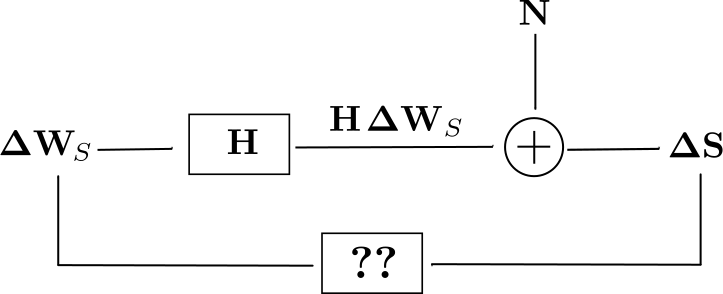
\includegraphics[scale = 0.5]{direct_model}
\caption{direct model schematic}
\label{fig: direct model}
\end{figure}

The problem is how to find $\Delta W$ for the measurement of $\Delta S$, so how to inverse the direct problem. A naive approach will be to discard the unknown noise and to just invert the known convolution product $H$, as represented in schematic \ref{fig: naive deconvolution}.

\begin{figure}[H]
\centering
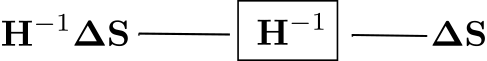
\includegraphics[scale = 0.5]{naive_deconvolution}
\caption{naive deconvolution schematic}
\label{fig: naive deconvolution}
\end{figure}

To support the explanation in this annex we can take the example of a spectroscopy (or 0$^{\mathrm{th}}$ harmonic) measurement of a 2 GHz sine wigner function. If we look at the estimated result $H^{-1}\Delta S$ in figure ... one can clearly remark that the estimator is dominated by only one oscillation. This result is clearly not reliable as it is sensible to small error perturbation as one can check if we apply to a different data set measured in the same condition and that do not seemed to show sensible difference, as tested on figure .... It also does not verify physical properties such as Pauli principle, which implies that the result plus the fremi function should be bounded between 0 and 1:

\begin{equation}
0 \leq f+\mathrm{fermi} \leq 1
\end{equation}

This behaviour is explained by the fact that deconvolution is an ill-posed problem. This means that the $H$ matrix that model the convolution has some zero or close to zero eigenvalues. This can be shown in the fourier space where the convolution is just the product by the fourier transform of the convolution function $h$ which posses some zeros. So inverting $H$ is equivalent to divide some Fourier component of $\Delta S$ per 0, and even if $H\Delta W$ vanishes for these points, the noise $N$ doesn't and the solution is completely dominated by these noise terms.

\section{The field}

%présenter le domaine

This problem of inverting an ill-posed problem is also present in other situation such as image deblurring, reconstructiion. We benefit from these developpement to adapt and apply it to our specific case.

\section{The Fourier space technique: Wiener filter}

%présenter technique wiener filtering

The first technique to overcome the problem presented in section \ref{The problem} is to filter the Fourier components of noise divided by zero. The idea is to find the optimum filter which by averaging on realization of the noise $N$ gives the minimum of the distance between filtered result $FH^{-1}\Delta S$ and the original signal $\Delta W$, this distance is:

\begin{equation}
<|| FH^{-1}\Delta S - \Delta W ||^{2}>
\end{equation}

and so by solving the equation

\begin{equation}
\frac{\mathrm{d}}{\mathrm{d}F}\left( <|| H^{-1}F\Delta S - \Delta W ||^{2}> \right) = 0
\end{equation}

and we find

\begin{equation}
F = \frac{HH^{\ast}}{HH^{\ast}+\left<\left|\frac{N}{\Delta W}\right|^{2}\right>} = \frac{1}{1+\left<\left|\frac{N}{H\Delta W}\right|^{2}\right>}
\end{equation}

\begin{itemize}
\item in the case of a convoluted signal higher than the noise $N\ll H\Delta W$, we get $\Delta S \sim H\Delta$ and so we don't need to filter since $H^{-1}\Delta S \sim \Delta W$ and this is the case because in this limit $F \sim 1$.
\item The other case is when the convoluted signal is smaller than the noise $H\Delta W\ll N$. This implies that we measure only noise $\Delta S \sim N$ so the filter has to suppress this term. And this is the case since $F \sim \left<\left|\frac{H\Delta W}{N}\right|^{2}\right> \ll 1$
\end{itemize}

To construct this filter we need two quantities first the noise spectrum $<|N|^{2}>$ which can be measured if we assumed a white noise and if we use repeated measurement. The second quantity is the spectrum of the solution $|\Delta W|^{2}$, but as it is the one we are looking for, we don't know it. So we need to use some hypothesis to approach the optimum filter. To do so the first one is that when $\Delta S \gg N$ we can assume $\Delta W \sim H^{-1}\Delta S$ and so the filter has the form:

\begin{equation}
F = \frac{1}{1+\left<\left|\frac{N}{\Delta S}\right|^{2}\right>}
\end{equation}

When $\Delta S \sim N$ we know that $H\Delta W \leq N \sim \Delta S$ so we assumed that there is a corner point where $\Delta W \leq \Delta W(\tau_{c}) \sim \frac{\Delta S(\tau_{c})}{H(\tau_{c})}  \sim \frac{N}{H(\tau_{c})}$ and that we use as a bound for our filter:

\begin{equation}
F = \frac{1}{1+\left|\frac{H(\tau_{c})}{H}\right|^{2}}
\end{equation}

We end up with the following filter

\begin{eqnarray}
F &=& \frac{1}{1+\left<\left|\frac{N}{\Delta S}\right|^{2}\right>} \mathrm{when} H \geq H(\tau_{c}) \\
  &=& \frac{1}{1+\left|\frac{H(\tau_{c})}{H}\right|^{2}} \mathrm{when} H \leq H(\tau_{c}) \\
\end{eqnarray}

The result on the example of the spectroscopy measurement and the whole wigner function of a 2 GHz sine is display in figure ...

%les barres d'erreur on a bruit blanc gaussien, on applique un filtre dessus, puis TF comme les points sont indépendants je suis sura que ça reste diagonal donc même barre d'erreur partout, mais elles sont filtrées. faut aussi expliquer ça.

\begin{figure}[H]
\centering
\includegraphics[scale = 0.5]{Wiener_deconvolution}
\caption{Wiener deconvolution schematic}
\label{fig: Wiener deconvolution}
\end{figure}

\section{The Bayesian framework}

The problem of the above technique is as we don't know the power spectrum of the solution, we are forced to use hypothesis that don't correspond to physical properties. To get a solution which verify known physical properties, we introduce a new problem formulation. The measurement is the mean of the probability distribution of $\Delta S$ knowing the searched quantity $\Delta W$ and the variance $V_{e}$ of Gaussian noise $N$.

\begin{equation}
p\left(\Delta S | \Delta W, V_{e} \right) = \exp\left(-\frac{1}{2}||\Delta S - H\Delta W||_{V_{e}}^{2}\right)
\end{equation}

But what we are looking for is $\Delta W$ so we are interested in the probability distribution of $\Delta W$ knowing the measurement $\Delta S$ and the noise variance $V_{e}$. Thanks to Bayes'formula we can link the two precedent probability distribution.

\begin{equation}
p\left(\Delta W |\Delta S , V_{e} \right)p\left(\Delta S\right) = p\left(\Delta S | \Delta W, V_{e} \right)p\left(\Delta W \right)
\end{equation}

So we can expressed the probability distribution of interest $p\left(\Delta W |\Delta S , V_{e} \right)$, thanks to the measurement with $p\left(\Delta S | \Delta W, V_{e} \right)$ and to a prior knowledge on the solution with $p\left(\Delta W \right)$.

\subsection{Posterior law maximization}

%présenter le framework Bayesian avec MAP

%un peu dire que ce qu'on cherche c'est le max de la loi de probabilité. qu'on peut dire comme a priori qu'on cherche le signal de norme 2 minimum et qu'on préviligie les petites énergies aux grandes. et donc on a juste besoin de trouver le minimum de -log(p) soit du critère J. et que ça on peut le donner analytiquement par ...

\begin{figure}[H]
\centering
\includegraphics[scale = 0.5]{MAP_deconvolution}
\caption{MAP deconvolution schematic}
\label{fig: MAP deconvolution}
\end{figure}

%aidez la présentation avec le direct sampling

%dire qu'on peut faire un tirage au sort pour avoir l'histogramme de valeurs qui suit la loi de la distribution a posteriori et montrer que ça donne le même résultat

%dire qu'on peut aussi donner des barres d'erreur en calculant tout simplement ...

\subsection{Unsupervised technique with joint posterior law}

%présenter le un-supervised avec JMAP

\begin{figure}[H]
\centering
\includegraphics[scale = 0.5]{JMAP_deconvolution}
\caption{JMAP deconvolution schematic}
\label{fig: JMAP deconvolution}
\end{figure}

%aidez la présentation avec la Monte-Carlo-Markov-Chain

\subsection{Box-constraint problem with projected gradiant}

%présenter la box-constraint et le gradient projeté

\begin{figure}[H]
\centering
\includegraphics[scale = 0.5]{ProjGrad_deconvolution}
\caption{Projected Gradient deconvolution schematic}
\label{fig: ProjGrad deconvolution}
\end{figure}

\subsection{outlook: toward a 2D treatment}

%mettre en perspective le full traitement 2D

\begin{figure}[H]
\centering
\includegraphics[scale = 0.5]{1D_deconvolution}
\caption{1D deconvolution schematic}
\label{fig: 1D deconvolution}
\end{figure}

\begin{figure}[H]
\centering
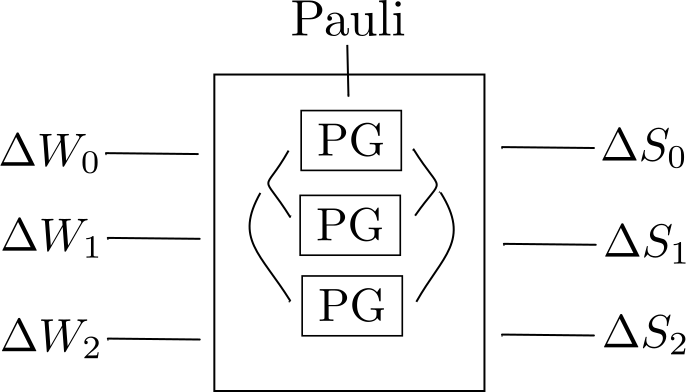
\includegraphics[scale = 0.5]{2D_deconvolution}
\caption{2D deconvolution schematic}
\label{fig: 2D deconvolution}
\end{figure}

\end{document}